\section{Datenbank Modelle}
In diesem Abschnitt werden die Grundlagen, der relationalen und Graph basierten Datenbank-Modell skizziert. Diese sind im Rahmen dieser Arbeit von wesentlicher Bedeutung. Schließlich vereint die in \compref{chap:db2graph} beschriebene Graph-Erweiterung sowohl Elemente des relationalen, als auch des Graph-Modells.

Um einen Überblick über die beiden Modelle zu geben, werden beide unter einem jeweiligen Aspekt des Modells einander gegenüber gestellt. Zu den Aspekten dieses Vergleichs gehören: 

\begin{itemize}
    \item Herkunft \& Verbreitung,
    \item Struktur \& Schema,
    \item Beziehungen und
    \item Abfragesprachen.
\end{itemize}

Die Beschränkung auf diese Aspekte wurde dabei vorgenommen, da ein tiefgreifender Vergleich beider Modelle über den Rahmen der Arbeit hinausgehen würde. Ziel dieses Abschnitts ist es lediglich einen kleinen Überblick über die verschiedenen Modelle zu geben. 

\subsection{Herkunft \& Verbreitung}
In diesem Unterabschnitt wird auf die Herkunft und aktuelle Verbreitung der beiden Modell eingegangen. Die Verbreitung wird dabei an der aktuellen Verbreitung von relationalen und Graph-Datenbanksystemen gemessen. 

\subsubsection{Relationales Modell}
Das relationale Modell hat seinen Ursprung in den 1970er Jahren \cite{rdbms_history}. Seine Grundlagen wurden dabei erstmals in \cite{codd_relational_model} von \citeauthor{codd_relational_model} umrissen. In den folgenden Jahren  wurde beim IBM Research unter dem Namen \textit{System R} ein erstes relationales Datenbanksystem entwickelt \cite{rdbms_history}. Es gilt dabei herauszustellen, dass die Paper die im Zuge der Forschung und Entwicklung am \textit{System R} veröffentlicht wurden, der Öffentlichkeit frei zur Verfügung gestellt wurden \cite{rdbms_history}. 

Heute haben relationale Datenbanksysteme eine große Verbreitung gefunden, siehe \autoref{}. So sollen nach \cite{db_engines_ranking_july} relationale Datenbanksysteme 72,7 \% des gesamten Datenbankmarktes ausmachen (Stand Juli 2021). Folglich kann dem relationalen Modell und relationalen Datenbanksystemen eine marktbeherrschende Rolle zugeschrieben werden.

% TODO INSERT PIE CHART

\subsubsection{Graph-Modell}
Das Graph- als Datenbank-Modell hat seinen Ursprung in der heutigen Form im Jahr 1999 \cite{gdbms}. Dabei wurde das Graph-Modell mit der Motivation entwickelt, vermeintliche Nachteile oder Probleme des relational Modells auszuräumen \cite{gdbms}.

Graphdatenbanksysteme und das Graph-Modell sind heute als vergleichbar junge Technologien sind heute noch nicht so weit verbreitet, wie beispielsweise, dass relationale Modell. Mit 1,7 \% Marktanteil ordnen sich Graph-Datenbanksysteme, noch weit hinter anderen Technologien ein, wie \textit{Document Stores}, \textit{Key-Values Stores} oder \textit{Wide column stores} \cite{db_engines_ranking_july}, siehe \autoref{}. Jedoch haben Graphdatenbanksysteme seit 2013 einen erheblichen Aufschwung in Popularität erfahren \cite{db_engines_ranking_july}. 

\subsection{Struktur \& Schema}
Im Rahmen dieses Abschnitts wird auf die vorhandenen Strukturen der Datenbankmodelle eingegangen. Darüber hinaus wird auch das zugrundeliegende Schema genauer erläutert. 

\subsubsection{Relationales Modell}
\label{datenmodelle:structure:relational}
Im Zentrum des relationalen Modells steht hierbei das sogenannte Informationsprinzip \cite{rdbms_history}. Dies beschreibt, dass alle Informationen in einer Datenbank ausschließlich in exakt einer Weise repräsentiert werden dürfen \cite{codd_relational_model}. Informationen werden dabei in Form von Tupeln und Relationen organisiert \cite{codd_relational_model}. Für deren Organisation stellen relationale Datenbanksysteme Tabellen, Spalten und Zeilen als Strukturen bereit \cite{rdbms_history}. So werden auf Basis des Informationsprinzips, alle Informationen als Werte in einer Zelle einer bestimmten Tabelle abgelegt \cite{rdbms_history}.

Das relationale Modell setzt bei der Datenhaltung allerdings ein striktes Schema voraus \cite{rdbms_book}. Schließlich fordert das Informationsprinzip, dass alle Informationen immer in genau einer Art und Weise repräsentiert werden müssen \cite{rdbms_history}. Es verlangt somit eine homogene Darstellung der Daten. Allerdings sind viele Daten in der realen Welt heterogen. Dies hat zu Folge, dass Daten einen sogenannten Normalisierungsprozess durchlaufen müssen \cite{rdbms_book}. Bei diesem Prozess werden die Daten in die sogenannte dritte Normalform (3NF) gebracht, wodurch jegliche Anomalien vermieden werden können \cite{rdbms_book}. So können letztendlich die Informationen einer Entität in einem homogenen Typschema abgebildet werden. 

\subsubsection{Graph-Modell}
Die Grundlage des Graph-Modells stellen sogenannte Vertexes und Edges dar, auf Deutsch Knoten und Kanten \cite{gdbms}. Diese Vertexes und Edges bilden dabei zusammen einen sogenannten Graphen. So werden in einem Graphen einerseits Entitäten in Form eines Knotens repräsentiert \cite{gdbms}. Anderseits bildet es auch explizit Beziehungen zwischen Entitäten mittels Kanten ab \cite{gdbms}. Darauf wird aber \autoref{datenmodelle:beziehungen}  weiter eingegangen.

Das Graph-Modell setzt im Gegensatz zum relationalen Modell auf ein flexibles Datenschema \cite{gdbms}. Dadruch unterstützt es den Umgang mit heterogenen Daten \cite{gdbms}. Denn anstatt einer strikten Typisierung der Entitäten -- durch Tabellen im relationalen Modell -- lassen sich die Daten im Graph-Modell anhand von Labels organisiert werden. Labels markieren dabei Knoten oder Kanten, die dieselbe oder eine ähnliche Rolle einnehmen. Sie sind in ihrer Funktion allerdings nicht mit Tabellen aus dem relationalen Modell vergleichbar. Dies liegt darin begründet, dass Entitäten mit einem bestimmten Label unterschiedliche Informationen aufweisen können. 

\subsection{Beziehungen}
\label{datenmodelle:beziehungen}
In diesem Abschnitt wird darauf eingegangen, wie und in welcher Form die Modelle mit Beziehungen zwischen Entitäten abbilden. 

\subsubsection{Relationales Modell}
Beziehungen im relationalen Modell lassen sich in die drei folgenden Kategorien unterteilen: 
\begin{itemize}
    \item \textit{one-to-one}, 
    \item \textit{one-to-many} (beziehungsweise \textit{many-to-one}) und 
    \item \textit{many-to-many}.
\end{itemize}
Je nachdem welche der drei Kategorien vorliegt, müssen im relationalen Modell die Beziehungen anders aufgelöst werden. Dabei spielen bei allen drei Kategorien die folgenden Begriffe eine Schlüsselrolle:
\begin{itemize}
    \item Primärschlüssel, 
    \item Sekundärschlüssel und
    \item Joins.
\end{itemize}

\section{Datenbanken (Deprecated)}
Im Rahmen dieses Kapitels zwei unterschiedliche Arten von \acl{dbms} erläutert. Zu diesen Arten gehören \acl{rdbms}, \acl{ddbms} und \acl{gdbms}. Im Zuge der Erläuterung der \acs{dbms} werden das Modell, die Geschichte sowie besondere Eigenschaften angesprochen. Ziel ist es dabei nicht die Modelle ausführlich bis in das kleinste Detail zu erklären. Stattdessen soll im Rahmen dieses Kapitels lediglich die grobe Herkunft, das Modell und die Funktionsweise der verschiedenen \acs{dbms}-Konzepte erläutert werden, sodass in den folgenden Kapiteln auf den hier beschriebenen Begriffen und Konzepten aufgebaut werden kann.   

\subsection{\acl{rdbms}s}
Bei dem relationalen Datenbankmanagementsystemen handelt es sich um eine verbreitetet und erprobte Art \acs{dbms}. Schließlich solche relationalen Systeme bereits seit einigen Jahren am Markt verfügbar. 

\subsubsection{Geschichte}
Das relationale Datenmodell auf dem alle relationalen Datenbankmanagementsysteme aufbauen, hat seinen Ursprung in den 1970er Jahren. Dort wurde es erstmals in \cite{codd_relational_model} beschrieben. Im Rahmen von \cite{codd_relational_model} umreist \citeauthor{codd_relational_model} ein Datenmodell, bei dem Informationen in Form von Tupeln und Relationen organisiert werden. Angelehnt an das von \citeauthor{codd_relational_model} skizzierte Datenmodell, wurden in den folgenden Jahren die ersten relationalen Datenbanksysteme entwickelt. 

\subsubsection{Modell}
Relationale Datenbanksysteme organisieren hierbei ihre Daten in Form von Tabellen (Relationen), Spalten und Zeilen (Tupeln). Tabellen stellen dabei immer einen bestimmten Entitätentyp dar z.B. ein Auto oder einen Autobesitzer. Diese Entitätentypen verfügen immer über ein oder mehrere fest definierte Attribute. Bei einem Auto könnten solche Attribute die Fahrzeugnummer, der Marke, das Modell und das Baujahr sein, siehe \autoref{tab:auto_table}. 

\begin{table}[h]
    \centering
    \begin{tabular}{c|c|c|c}
    \hline
    \rowcolor[HTML]{EFEFEF} 
    \multicolumn{1}{l|}{\cellcolor[HTML]{EFEFEF}\textbf{Fahrzeugnummer}} & \multicolumn{1}{l|}{\cellcolor[HTML]{EFEFEF}\textbf{Marke}} & \multicolumn{1}{l|}{\cellcolor[HTML]{EFEFEF}\textbf{Model}} & \multicolumn{1}{l}{\cellcolor[HTML]{EFEFEF}\textbf{Baujahr}} \\ \hline
    FZ-123456789 & Toyota & Starlet & 1997 \\
    FZ-234567890 & Nissan & Leaf & 2018 \\
    FZ-345678912 & VW & ID3 & 2020 \\
    FZ-456789123 & Ford & Fiesta & 2001 \\
    ... & ... & ... & ... \\ \hline
    \end{tabular}
    \caption{Auto Tabelle}
    \label{tab:auto_table}
\end{table}

Es ist dabei auch möglich, Beziehungen zwischen unterschiedlichen Entitätentypen (Tabellen) aufzubauen. Hierbei unterstützen relationale Datenbanksysteme die folgenden Typen von Entitätsbeziehungen: 
\begin{itemize}
    \item \textit{one-to-one}, 
    \item \textit{one-to-many} bzw. \textit{many-to-one} und 
    \item \textit{many-to-many}.
\end{itemize}
\textit{One-to-one}- und \textit{one-to-many}-Beziehungen lassen sich dabei ohne großen Aufwand umsetzen. Hierbei muss lediglich eine neue Spalte für Fremdschlüssel in eine der Tabellen eingefügt werden. Dieser verweist auf das identifizierende Attribut -- den Primärschlüssel -- der anderen Tabelle. Die Abstraktion von \textit{many-to-many}-Beziehungen ist hierbei etwas aufwändiger. Dabei muss eine Auflösungstabelle zwischen den zwei Tabellen aufgebaut werden, deren Entitätstypen in einer \textit{many-to-many}-Beziehung stehen. So wäre es beispielsweise möglich eine Besitz-Beziehung zwischen Autos und allen aktuellen und ehemaligen Besitzern aufzubauen. Diese Auflösungstabelle könnte dabei in Form eines Kfz-Registers abstrahiert werden, siehe \autoref{fig:rdbms_m2m}.

\begin{figure}[h]
    \centering
    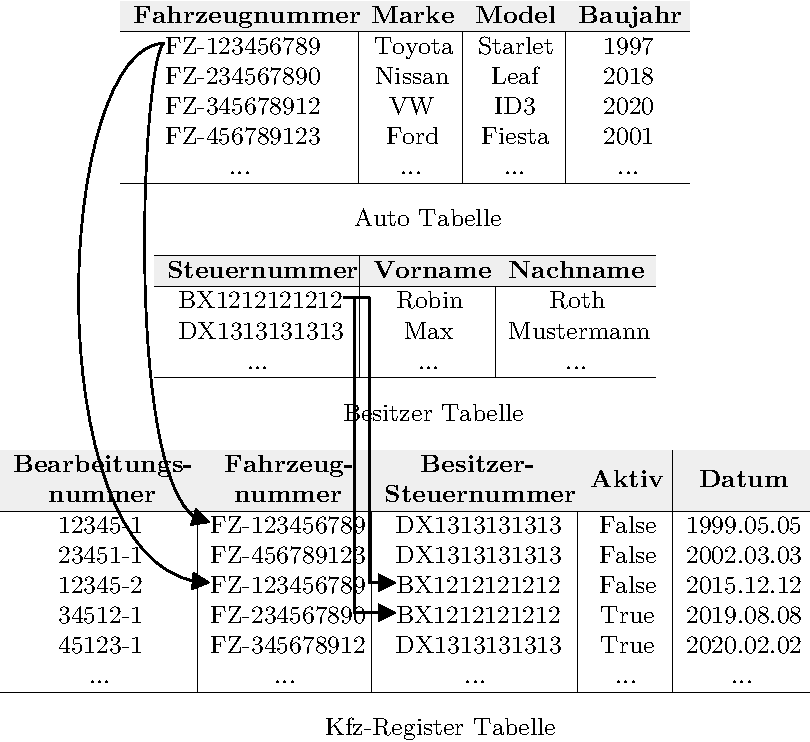
\includegraphics[width=\textwidth]{images/many-to-many.pdf}
    \caption{Beispiel RDBMS many-to-many-Beziehungen}
    \label{fig:rdbms_m2m}
\end{figure}

\subsubsection{SQL}
Über das Konzept des relationale Konzept der Datenbanken hinaus, gilt es die Abfragesprache SQL herauszustellen. Die Abfragesprache wurde als relationale Sprachen entworfen \cite{sql_history}. Dies geschah in Reaktion auf das von \citeauthor{codd_relational_model} beschriebene relationale Modell \cite{sql_history}. Darüber hinaus gilt nach \cite{sql_history} SQL als eine einfach zu erlernende Sprache. 

SQL nimmt heute im Umfeld von \acs{rdbms} eine große Rolle ein. Bekannte relationale Datenbanksysteme wie DB2, PostgreSQL, Oracle Database und Microsoft SQL Server unterstützen alle die Abfragesprache SQL. Einige von den aufgeführten Systemen tragen die Abfragesprache sogar im Namen. Dabei gilt es allerdings zu beachten, dass sich die angesprochenen Datenbanksysteme alle durch verschiedene SQL-Dialekte auszeichnen. 

Die SQL als relationale Sprache ermöglicht es Datenstrukturen in Form von Tabelle zu definieren. Für das Schreiben der Daten in die Tabelle sowie das Auslesen, Ändern und Löschen bietet SQL ebenfalls Operationen an. Mit Primär- und Fremdschlüssel verfügt der SQL-Sprachumfang auch über Konstrukte zur Abbildung von Entitätsbeziehungen. 

\subsection{\acl{gdbms}s}



